\section{Mikrocontroller}\label{Appendix:Mikrocontroller}

\subsection{Fuse Bits}

\subsubsection{Brown-out-Detection}\label{Appendix:Brown-out-Detection}

\begin{figure}[H]
	\centering
	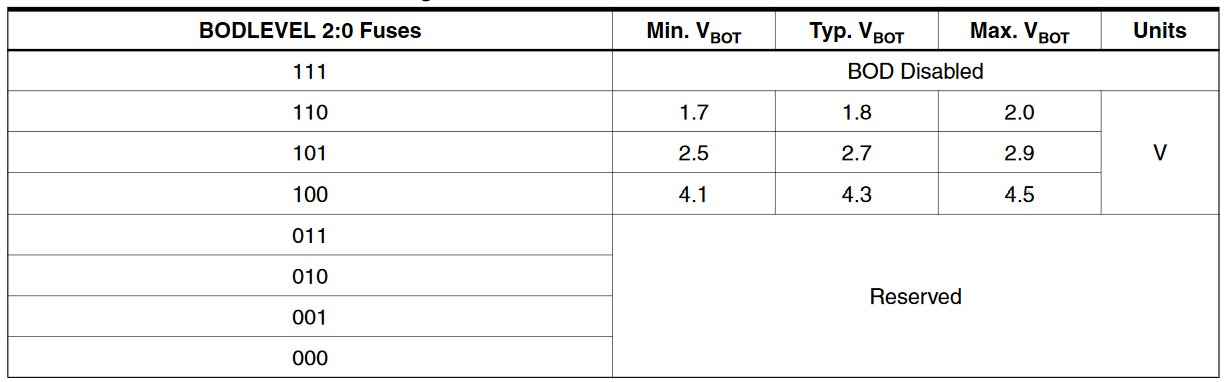
\includegraphics[width=0.7\textwidth]{graphics/Tabelle_BoD}
	\caption{Tabelle Brown-out-Detection.}
	\label{fig:Tabelle_BoD}
\end{figure}

\todo{cite: Datenblatt Atmega 2560, Seite 361}

\subsubsection{Full Swing Crystal Oscillator}\label{Appendix:Full_Swing _Crystal_Oscillator}

\begin{figure}[H]
	\centering
	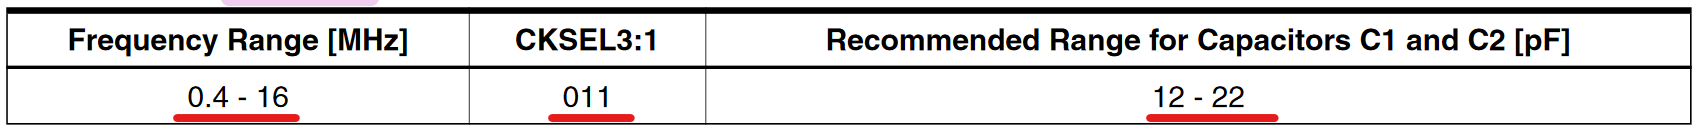
\includegraphics[width=0.7\textwidth]{graphics/Tabelle_Crystal}
	\caption{Tabelle Frequenzbereich Crystal Oszillator.}
	\label{fig:Tabelle_Crystal}
\end{figure}

\todo{cite: Datenblatt Atmega 2560, Seite 43}

\begin{figure}[H]
	\centering
	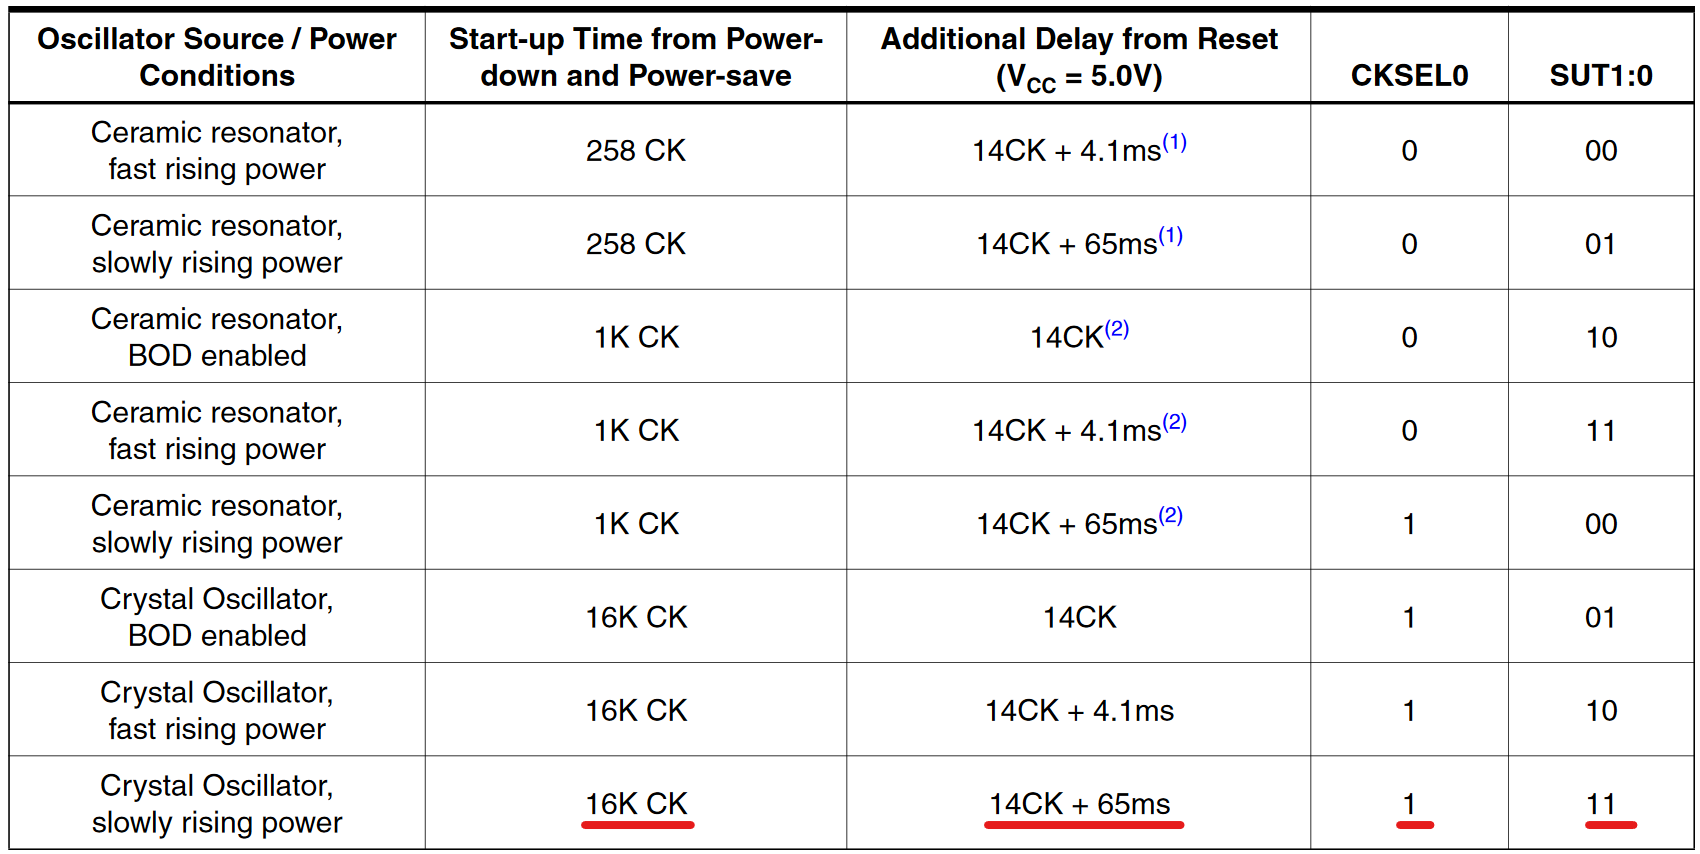
\includegraphics[width=0.7\textwidth]{graphics/Tabelle_Crystal2}
	\caption{Tabelle Aufstartzeit.}
	\label{fig:Tabelle_Crystal2}
\end{figure}

\todo{cite: Datenblatt Atmega 2560, Seite 43}

\subsubsection{Bootloader-Speicherplatz}\label{Appendix:Bootloader-Speicherplatz}

\begin{figure}[H]
	\centering
	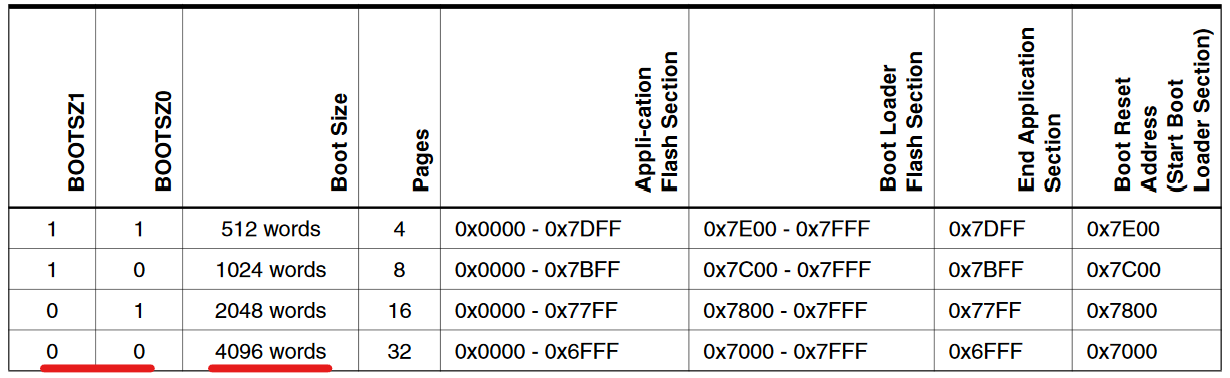
\includegraphics[width=0.7\textwidth]{graphics/Tabelle_Bootloader}
	\caption{Tabelle Bootloader Speicherplatz.}
	\label{fig:Tabelle_Bootloader}
\end{figure}

\todo{cite: Datenblatt Atmega 2560, Seite 320}

\subsubsection{Memory-Lock Bootloader}

\begin{figure}[H]
	\centering
	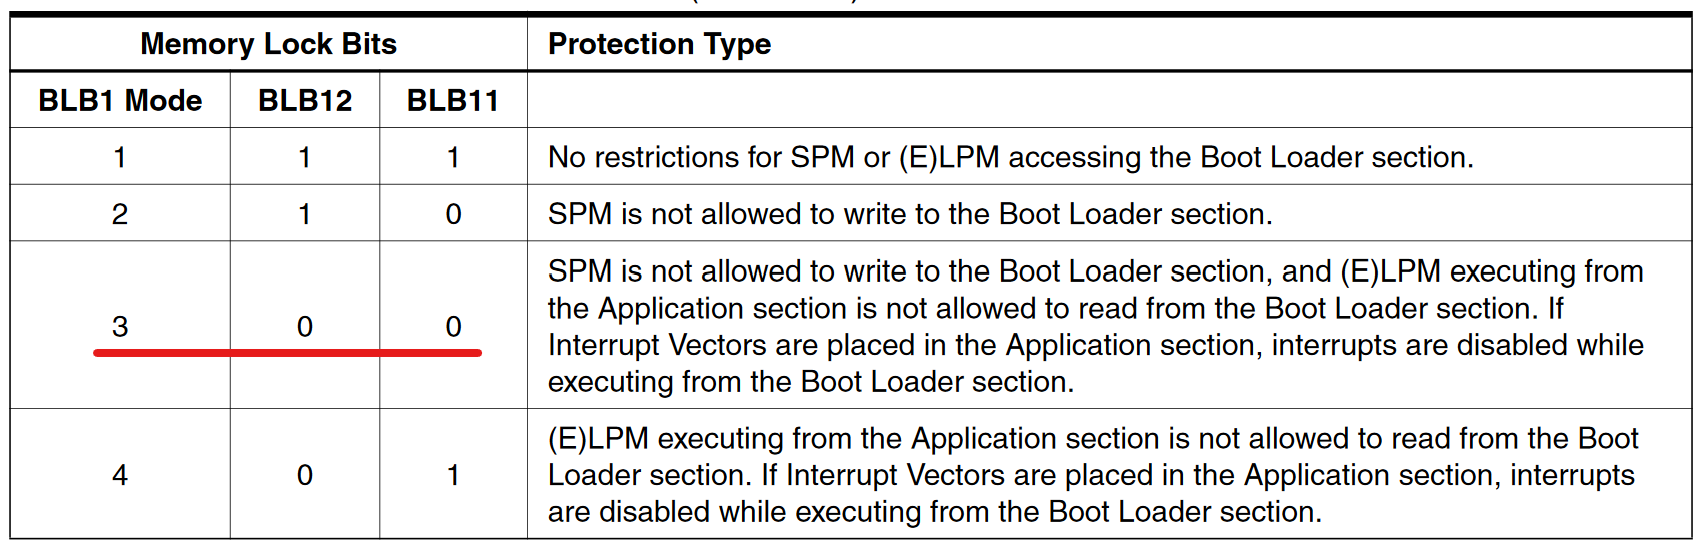
\includegraphics[width=0.7\textwidth]{graphics/Tabelle_Memory_Lock}
	\caption{Tabelle Memory Lock.}
	\label{fig:Tabelle_Memory_Lock}
\end{figure}

\todo{cite: Datenblatt Atmega 2560, Seite 326}

\subsection{Atmel Studio}

\subsubsection{Fuse Bits}

\begin{figure}[H]
	\centering
	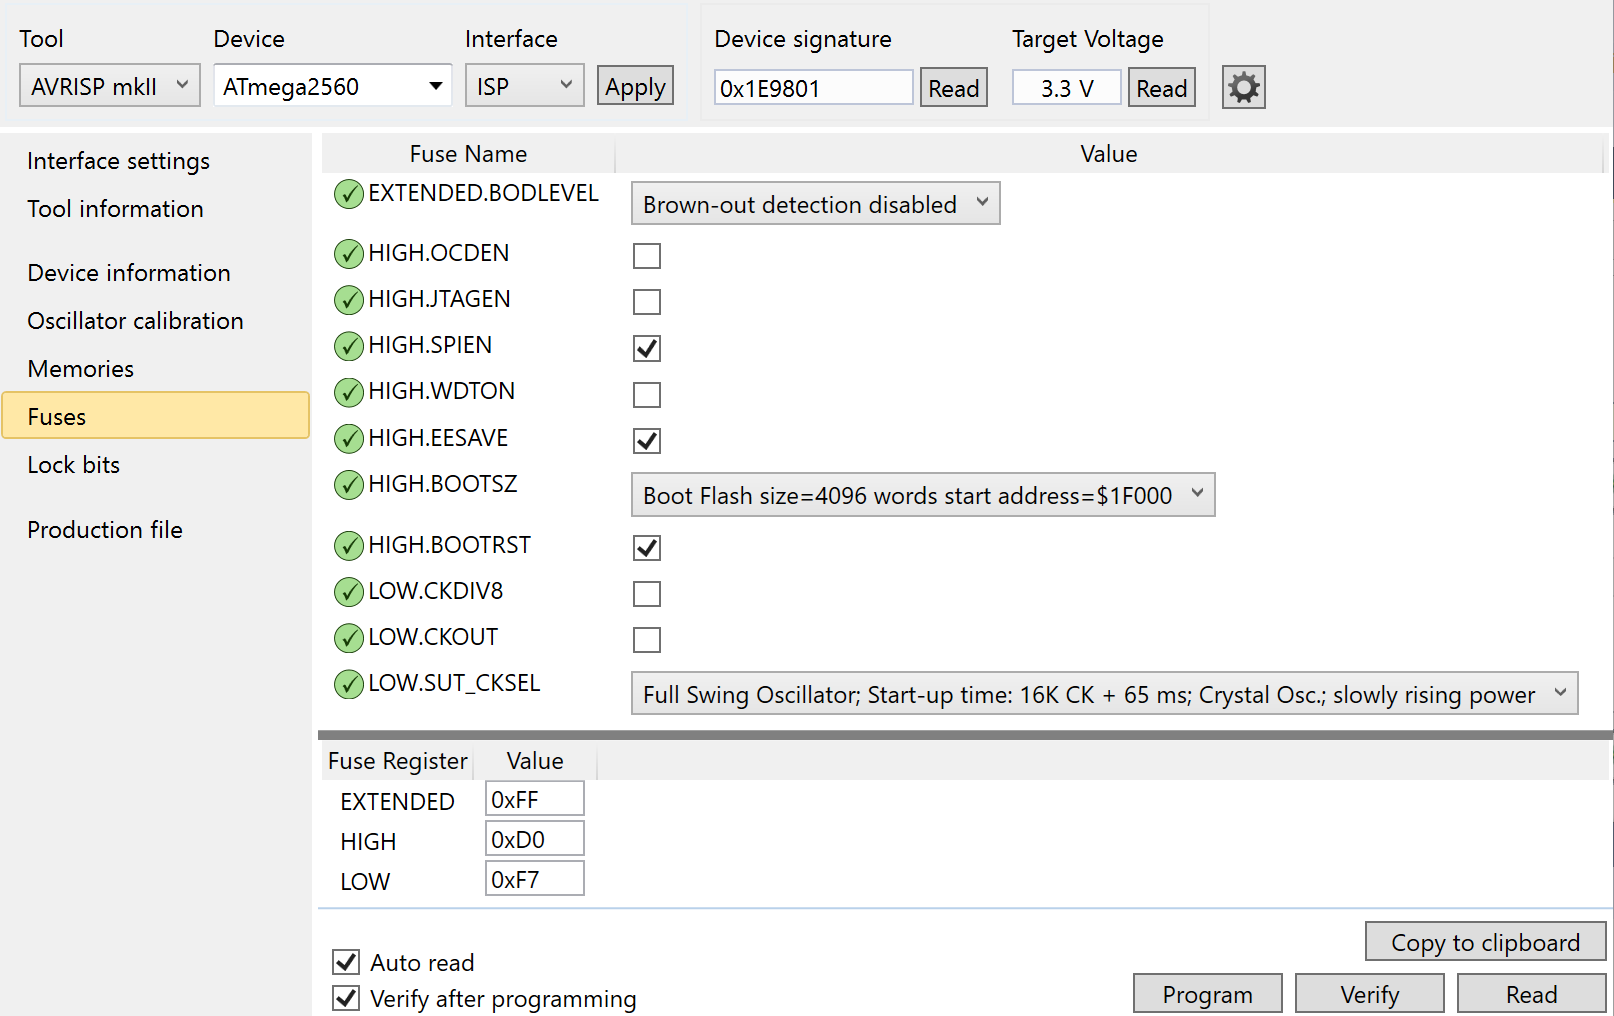
\includegraphics[width=\textwidth]{graphics/AtmelStudio_Fuses}
	\caption{Fuse-Bits Atmega2560.}
	\label{fig:AtmelStudio_Fuses}
\end{figure}

\subsubsection{Lock Bits}

\begin{figure}[H]
	\centering
	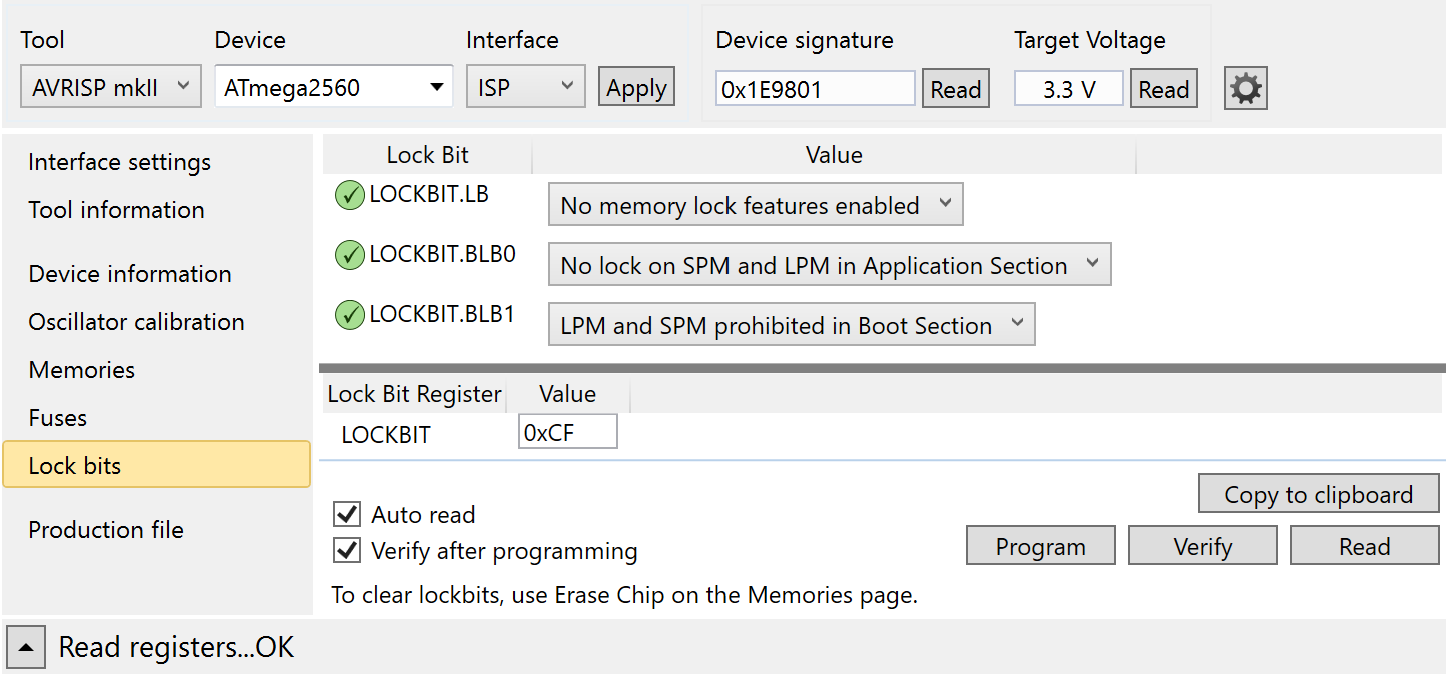
\includegraphics[width=\textwidth]{graphics/AtmelStudio_Locks}
	\caption{Lock-Bits Atmega2560.}
	\label{fig:AtmelStudio_Locks}
\end{figure}

\subsubsection{Einbinden AVRdude und stk500v2 (wiring)}

\begin{figure}[H]
	\centering
	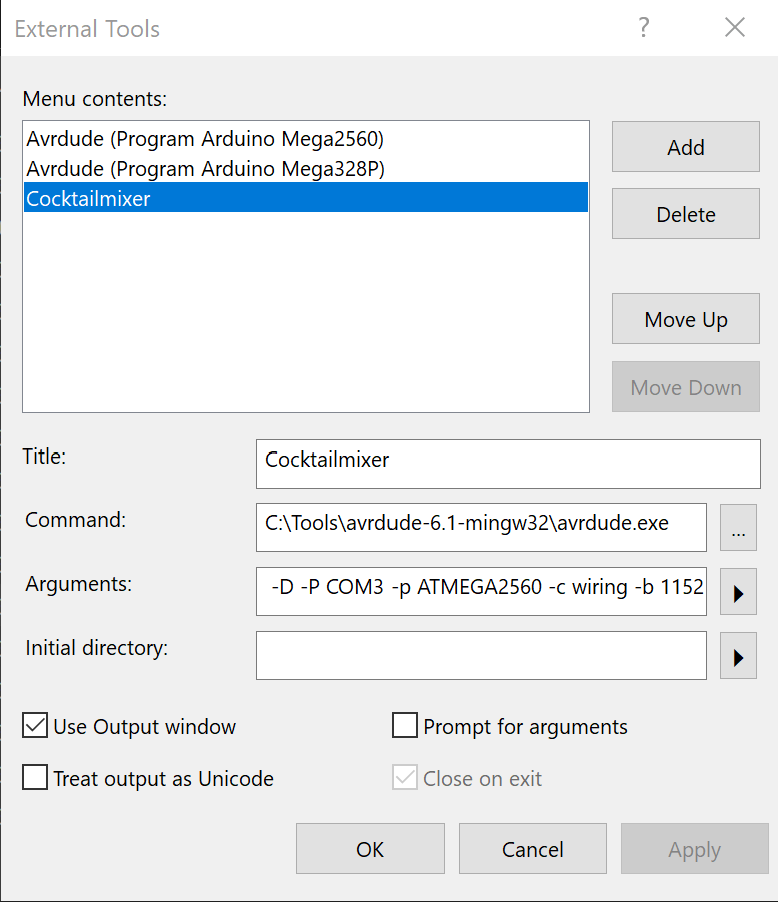
\includegraphics[width=0.5\textwidth]{graphics/AtmelStudio_External_Tools}
	\caption{External Tools Atmega2560.}
	\label{fig:AtmelStudio_External_Tools}
\end{figure}

\subsubsection{Bootloader ''Brennen''}

\begin{figure}[H]
	\centering
	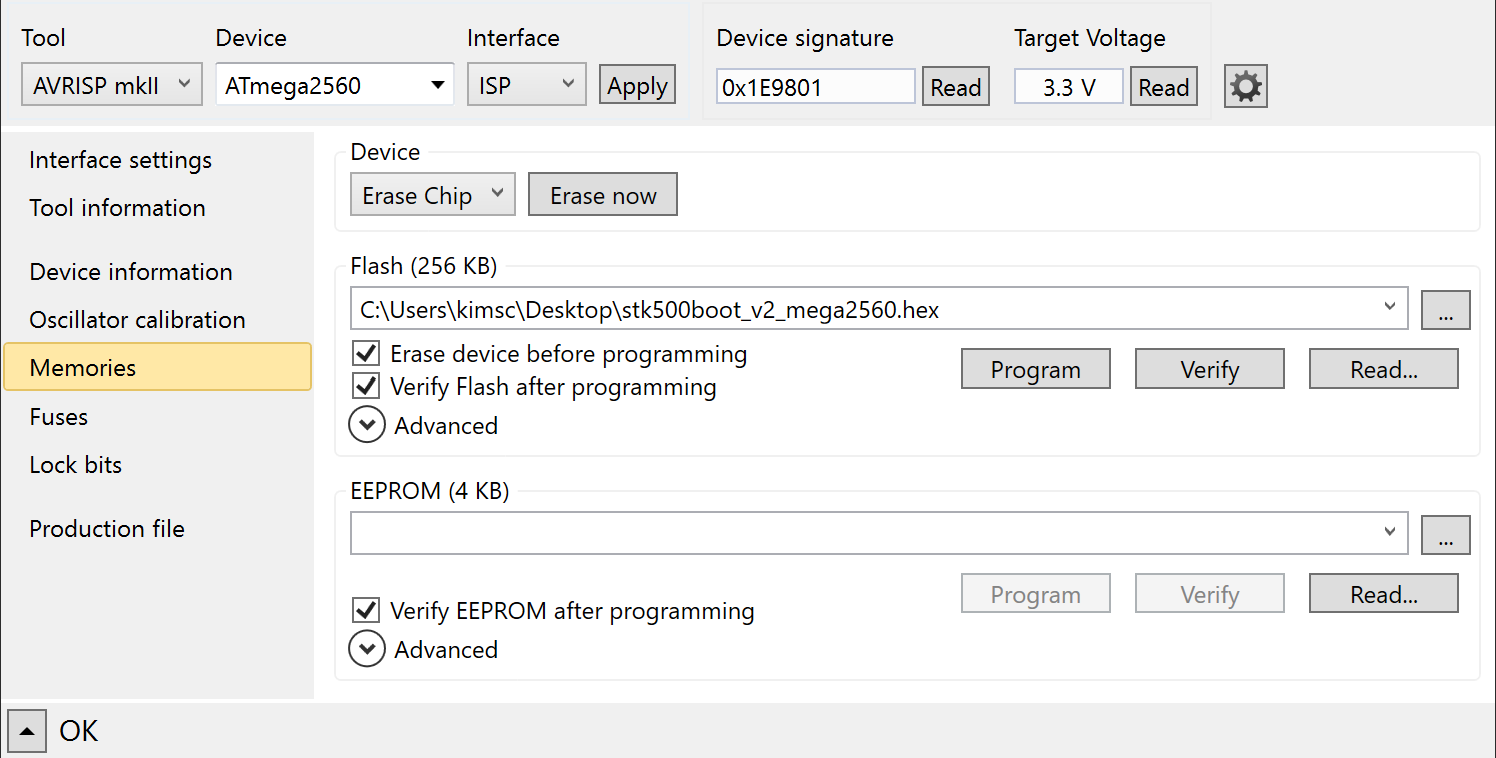
\includegraphics[width=\textwidth]{graphics/AtmelStudio_Program_Bootloader}
	\caption{Bootloader brennen.}
	\label{fig:AtmelStudio_Program_Bootloader}
\end{figure}

\subsection{Inbetriebnahme Mikrocontroller}

\subsubsection{Schwingung 16MHz Quarz}

\begin{figure}[H]
\center
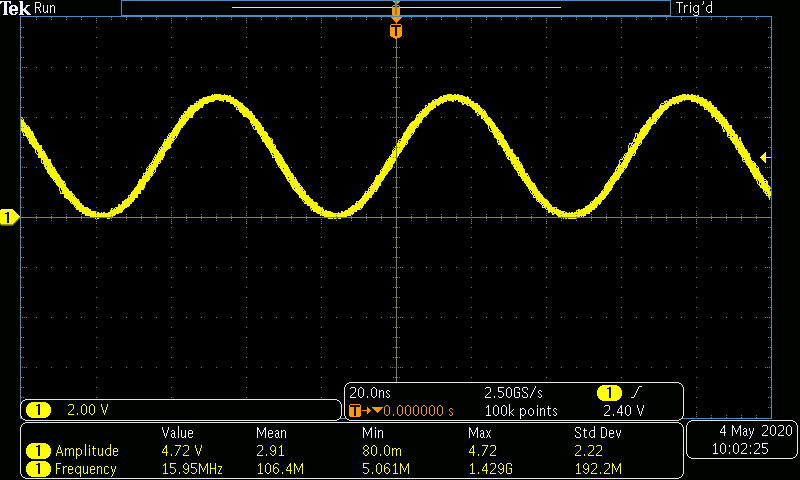
\includegraphics[width = 0.8\textwidth]{graphics/Crystal_Swing}
\caption{Schwingung des Oszillators}
\label{fig:Crystal_Swing}
\end{figure}

\subsection{Speicherorganisation}

\subsubsection{Doubly Dynamic Linked List}\label{Appendix:Lists}

In Abbildung \ref{fig:Doubly_Linked_List_2_0} wird nur der start-Pointer (head) initialisiert, ohne auf ein Element zu zeigen (NULL). Sobald der benötigte Speicherplatz des Elementes alloziiert wurde, wird der Zeiger auf die angelegte Struktur (Element) gelegt. Dem Head-Zeiger wurde nun ein Element zugewiesen und der Beginn der Liste wurde definiert.

\begin{figure}[h!]
	\centering
	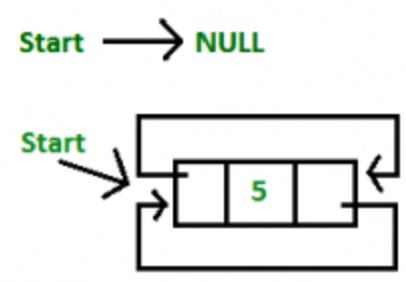
\includegraphics[width=0.5\textwidth]{graphics/Doubly_Linked_List_2_0}
	\caption{Doppelt verkettete Liste mit zwei Elementen.}
	\label{fig:Doubly_Linked_List_2_0}
\end{figure}

\todo{cite Bild:https://www.geeksforgeeks.org/doubly-circular-linked-list-set-1-introduction-and-insertion/}

Abbildung \ref{fig:Doubly_Linked_List_2_1} zeigt eine bestehende Liste mit zwei Elementen. Ein drittes Element soll am Schluss eingefügt werden. Dazu muss zuerst der Speicherplatz für das neue Element alloziiert werden (Data, next, prev). Danach können die Zeiger der bestehenden Elemente (in diesem Falle noch head und tail) umgelegt werden und die Zeiger des neuen Elementes auf das vorhergehende und nächste Element gelegt werden. Auch der tail-Zeiger muss nun auf das neue Element gelegt werden.

\begin{figure}[h!]
	\centering
	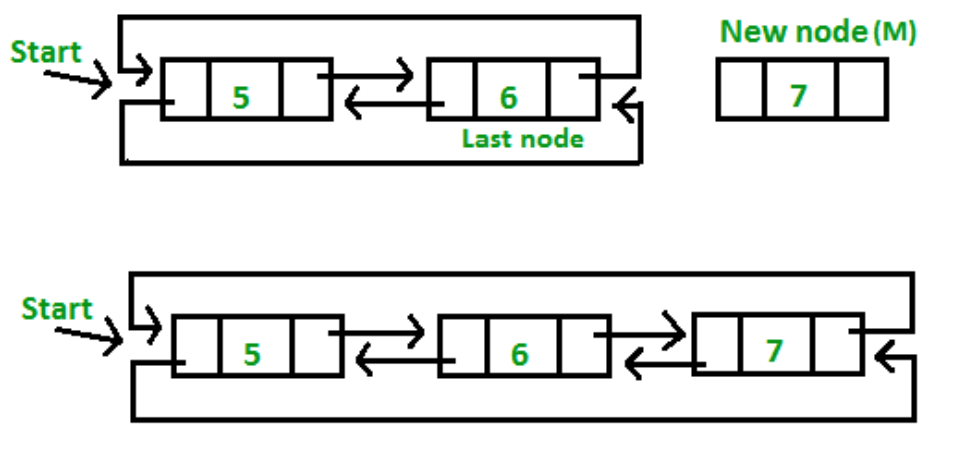
\includegraphics[width=0.5\textwidth]{graphics/Doubly_Linked_List_2_1}
	\caption{Doppelt verkettete Liste mit zwei Elementen.}
	\label{fig:Doubly_Linked_List_2_1}
\end{figure}

\todo{cite Bild:https://www.geeksforgeeks.org/doubly-circular-linked-list-set-1-introduction-and-insertion/}

Abbildung \ref{fig:Doubly_Linked_List_2_2} zeigt ebenfalls eine bestehende Liste mit zwei Elementen. Ein drittes Element soll am Beginn eingefügt werden. Dazu muss zuerst der Speicherplatz für das neue Element alloziiert werden (Data, next, prev). Danach können die Zeiger der bestehenden Elemente (in diesem Falle noch head und tail) umgelegt werden und die Zeiger des neuen Elementes auf das vorhergehende und nächste Element gelegt werden. Auch der head-Zeiger muss nun auf das neue Element gelegt werden.

\begin{figure}[h!]
	\centering
	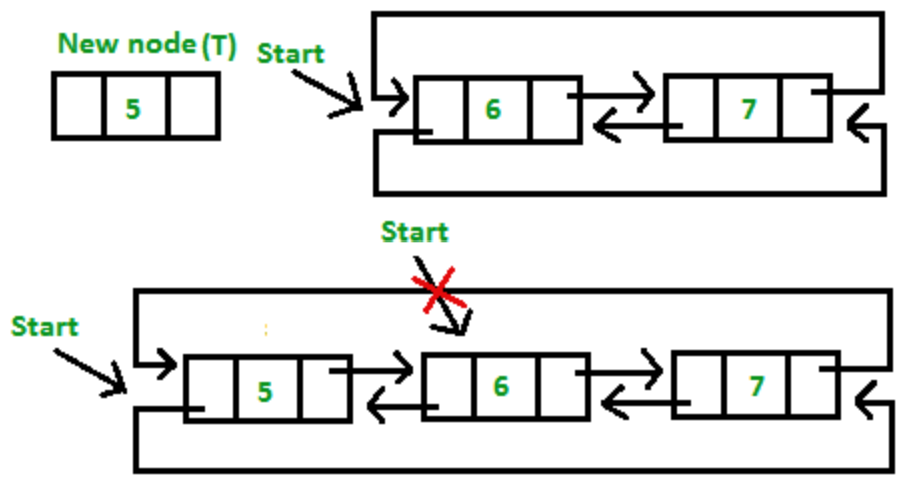
\includegraphics[width=0.5\textwidth]{graphics/Doubly_Linked_List_2_2}
	\caption{Doppelt verkettete Liste mit zwei Elementen.}
	\label{fig:Doubly_Linked_List_2_2}
\end{figure}

\todo{cite Bild:https://www.geeksforgeeks.org/doubly-circular-linked-list-set-1-introduction-and-insertion/}

Abbildung \ref{fig:Doubly_Linked_List_2_3} zeigt eine bestehende Liste mit vier Elementen. Ein fünftes Element soll in der Mitte eingefügt werden. Dazu muss zuerst der Speicherplatz für das neue Element alloziiert werden (Data, next, prev). Danach können die Zeiger der bestehenden Elemente umgelegt werden und die Zeiger des neuen Elementes auf das vorhergehende und nächste Element gelegt werden.

\begin{figure}[h!]
	\centering
	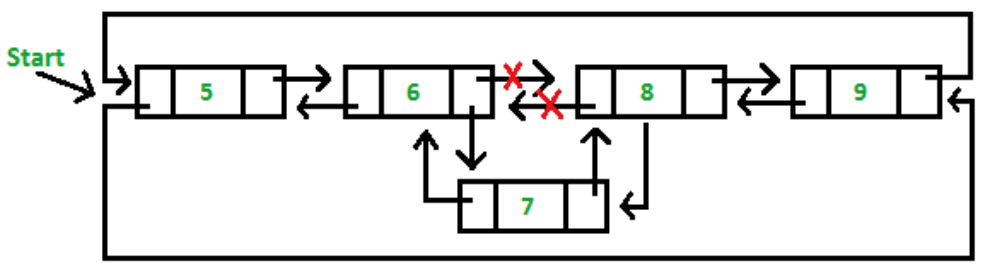
\includegraphics[width=0.5\textwidth]{graphics/Doubly_Linked_List_2_3}
	\caption{Doppelt verkettete Liste mit zwei Elementen.}
	\label{fig:Doubly_Linked_List_2_3}
\end{figure}

\todo{cite Bild:https://www.geeksforgeeks.org/doubly-circular-linked-list-set-1-introduction-and-insertion/}